


%......................................
\subsubsection*{Manifactured solution}

This benchmark begins by postulating a polynomial solution 
to the 3D Stokes equation \cite{dobo04}:
\begin{equation}
\vec{\upnu}(x,y,z)
=
\left(
\begin{array}{c}
x+x^2+xy+x^3y \\
y + xy + y^2 + x^2 y^2\\
-2z - 3xz - 3yz - 5x^2 yz
\end{array}
\right)
\label{eqbur2}
\end{equation}
and
\begin{equation}
p(x,y,z) = xyz + x^3 y^3z - 5/32
\end{equation}
The corresponding right-hand side is computed in Section~\ref{mms3}.
The domain is a unit cube and velocity boundary conditions
simply use Eq. (\ref{eqbur2}).
Note that the pressure fulfills $\int_\Omega p(x,y,z) dV = 0.$

\begin{center}
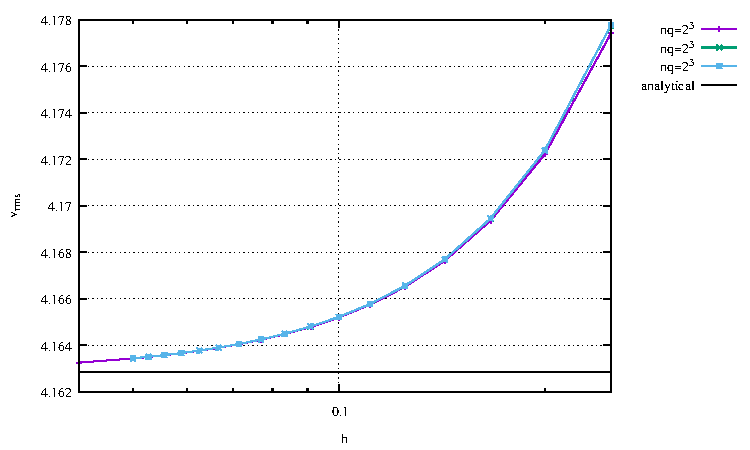
\includegraphics[width=8cm]{python_codes/fieldstone_82/results/mms/vrms.pdf}
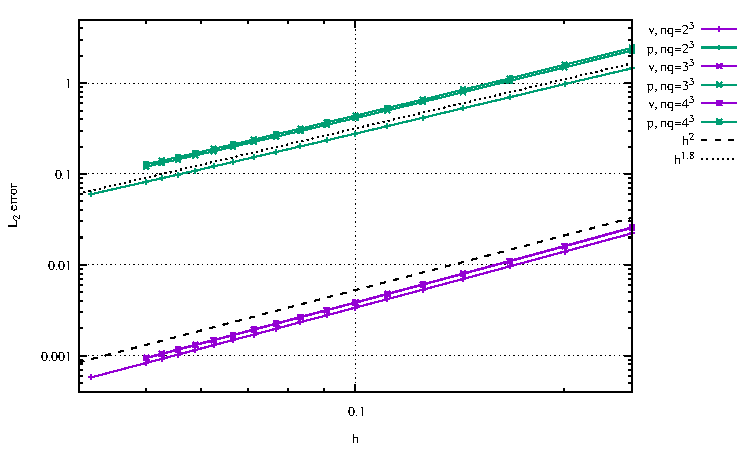
\includegraphics[width=8cm]{python_codes/fieldstone_82/results/mms/conv.pdf}\\
{\captionfont Results obtained for three levels of quadrature, with $\beta=0$ (i.e.
viscosity is constant and equal to 1).}
\end{center}

Somewhat surprisingly, the pressure convergence is not exactly quadratic but seems to be
around 1.8. Also, the $2\times 2\times 2$ 
quadrature yields better results than the $3\times 3\times 3$ or $4\times 4 \times 4$.

%......................................
\subsubsection*{Stokes sphere}

\begin{center}
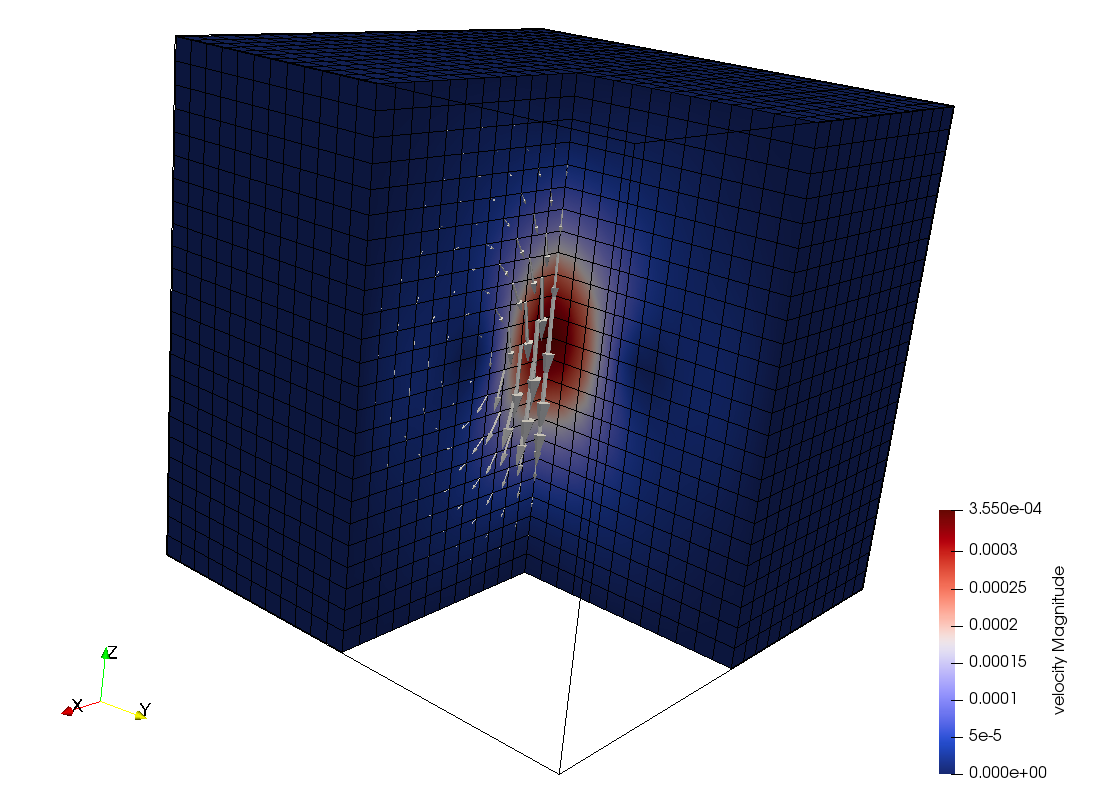
\includegraphics[width=7.5cm]{python_codes/fieldstone_82/results/sphere/vel}
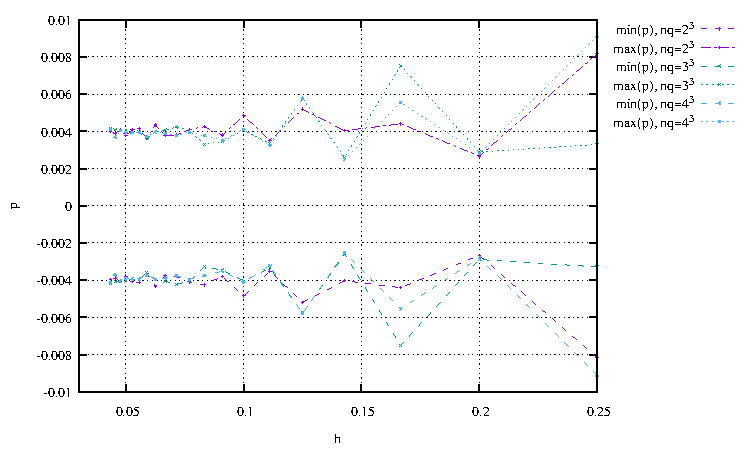
\includegraphics[width=7.5cm]{python_codes/fieldstone_82/results/sphere/p}\\
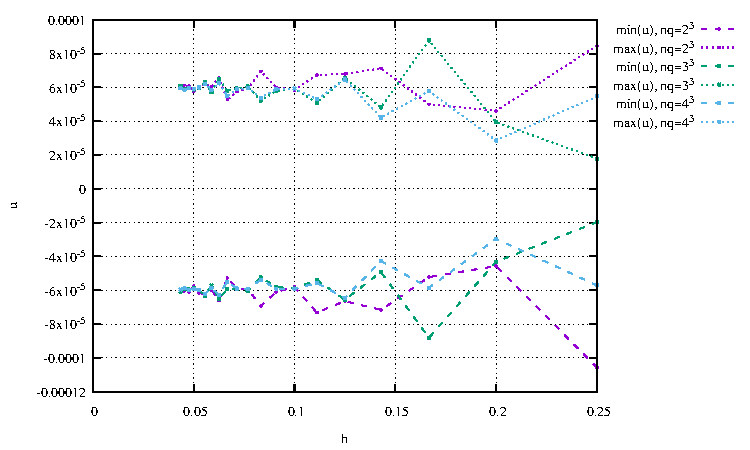
\includegraphics[width=5cm]{python_codes/fieldstone_82/results/sphere/u}
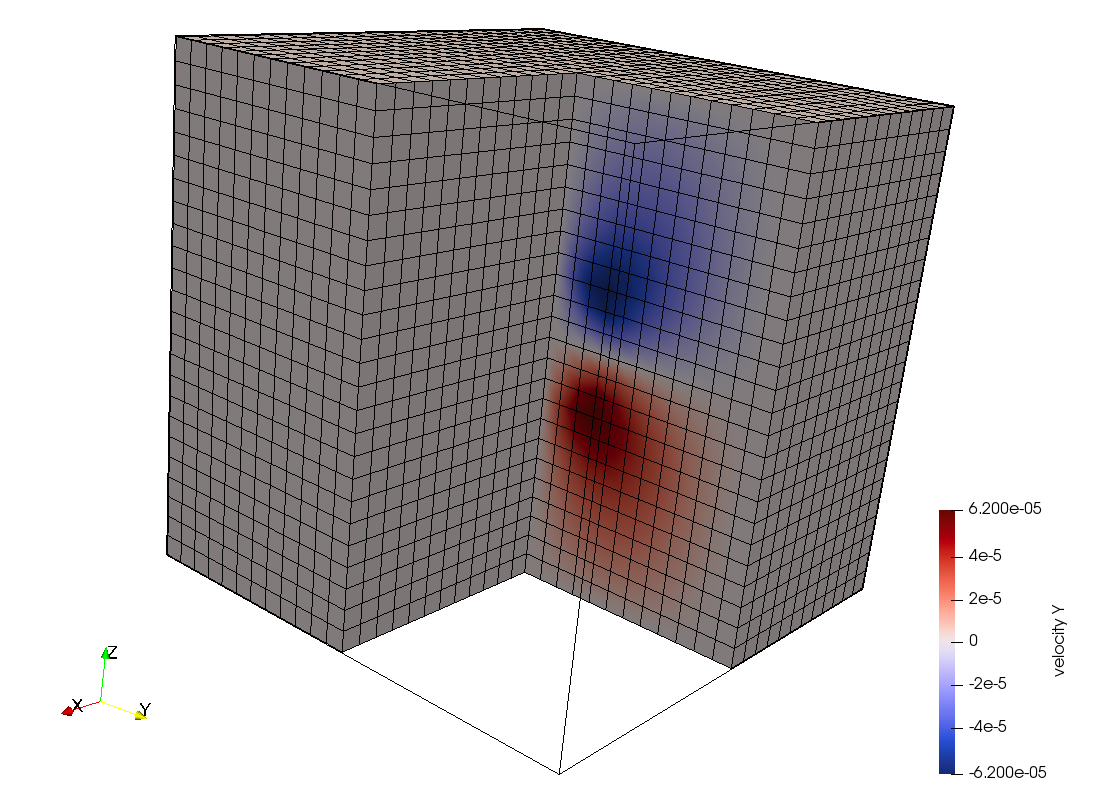
\includegraphics[width=5cm]{python_codes/fieldstone_82/results/sphere/v}
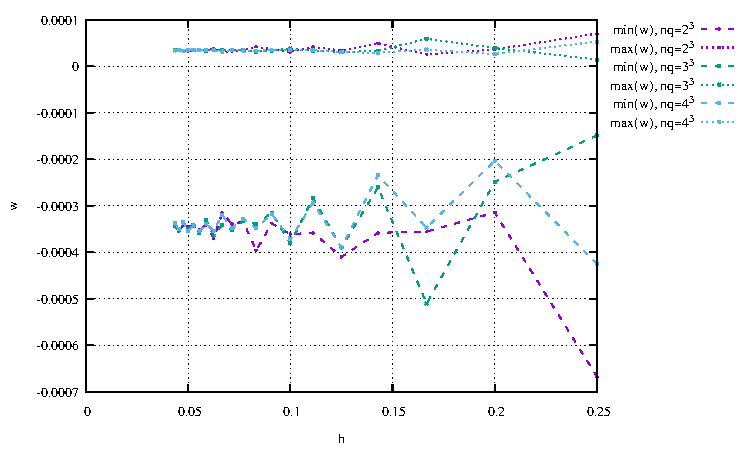
\includegraphics[width=5cm]{python_codes/fieldstone_82/results/sphere/w}\\
{\captionfont Resolution $24\times 24\times 24$. Quadrature $2\times 2 \times 2$.}
\end{center}


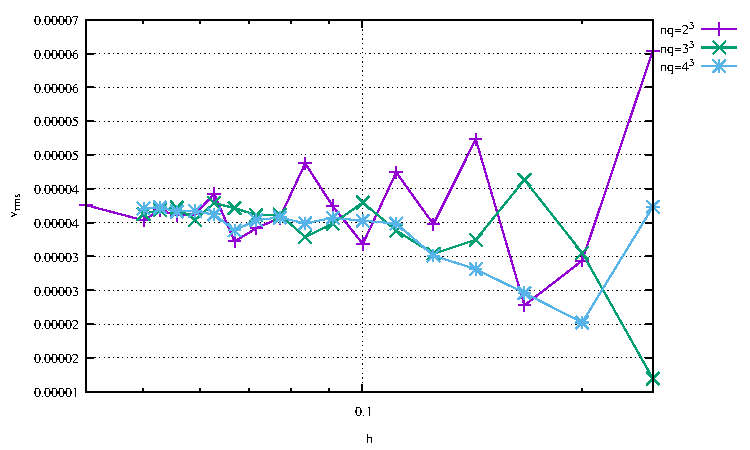
\includegraphics[width=8cm]{python_codes/fieldstone_82/results/sphere/vrms.pdf}



